\documentclass{article}
\usepackage{fancyhdr}
\usepackage{amsmath}
\usepackage{amsthm}
\usepackage{accents}
\usepackage{amssymb}
\usepackage{graphicx}
\usepackage{float}
\usepackage{subcaption}
\usepackage{hyperref}
\usepackage{listings}
\usepackage{color}
\usepackage{tikz}
\usepackage{pgfplots}
\usepackage{pgfplotstable}
\usepackage{listings}
\usepackage{color}
\usepackage{tikz}
\usepackage{amsthm}
\usepackage{soul}
\usepackage[margin=15mm]{geometry}
\usepackage[makeroom]{cancel}

\definecolor{dkgreen}{rgb}{0,0.6,0}
\definecolor{gray}{rgb}{0.5,0.5,0.5}
\definecolor{mauve}{rgb}{0.58,0,0.82}
\hypersetup{colorlinks=true,linkcolor=blue, linktocpage}
% Set up fancy header
\pagestyle{fancy}
\fancyhf{} % Clear default header and footer
\rhead{Keith Wesa} % Right header
\lhead{STAT 381 - Written Homework 2} % Left header
\rfoot{Page \thepage} % Right footer

\author{Keith Wesa}
\title{STAT 381 - Written Homework 2}
\date{\today}

\begin{document}
\section*{Question 1}
\subsection*{1.}
\textbf{Question:} Suppose Chester performs two calculations on the same random variable X: (a) he finds
the variance of a random variable; (b) he finds the variance of a (random variable times
some quantity). In your own words, explain why these two values will not be the same.

\begin{itemize}
    \item[] \textbf{Answer} 
    \item \textbf{Definition:} The variance of a random variable is a measure of how much the values of the random variable differ from the mean. 
    it's the average of the squared differences from the mean. Represented as $\sigma^2 = E[(X - \mu)^2]$
    \item \textbf{In Context:} In a discrete probability distribution, the variance of a random variable is the \textbf{Sum} of the squared differences from the mean.
    Since, it is a sum we need to take each value by themselves.
    \item \textbf{Equation}
    \begin{equation*}
        \sigma^2 = \sum_{i=1}^{n} (x_i - \mu)^2 \cdot P(x_i)
        \end{equation*}
\end{itemize}
\section*{Question 2}
Mary investigates two random variables, $X$ and $Y$ , where $Y = X^4$. She finds that
$E(XY ) = 0$, $E(X) = 0$, and $E(Y) = 4$.

\subsection*{(a)}
\textbf{Question:} Using this information, find $COV(X, Y)$
\begin{itemize}
    \item[] \textbf{Answer} 
    \item \textbf{Definition:} The covariance of two random variables is a measure of how much the two random variables vary together. 
    \item \textbf{Equation}
    \begin{equation*}
        \begin{aligned}
        &COV(X, Y) = E(XY) - E(X)E(Y) \\
        &\text{ or } \\
        &COV(X, Y) = E(XY) - \mu_X \mu_Y \\
        &\text{ where } \mu_X = E(X) \text{ and } \mu_Y = E(Y)
        \end{aligned}
        \end{equation*}
    \item \textbf{Given:} $E(XY) = 0$, $E(X) = 0$, and $E(Y) = 4$
    \begin{align*}
        COV(X, Y) &= E(XY) - E(X)E(Y)\\
        &= 0 - 0 \cdot 4\\
        &= 0
    \end{align*}
    \textbf{Conclusion:} The covariance of $X$ and $Y$ is 0.
\end{itemize}

\subsection*{(b)}
\textbf{Question:} In your onw words, describe the association between $X$ and $Y$.
\begin{itemize}
    \item[] \textbf{Answer: } The association between $X$ and $Y$ is 0. This means that the two random variables are not associated with each other.
\end{itemize}

\subsection*{(c)} \textbf{Question:} Are X and Y independent? Explain your answer using your own words. Include a
statement about your covariance calculation in your answer. (You do NOT need to
complete any calculations to answer this question.)
\begin{itemize}
    \item[] \textbf{Answer: } Yes, $X$ and $Y$ are independent. This is because the covariance of $X$ and $Y$ is 0. This means that the two random variables are not associated with each other.
\end{itemize}   
\section*{Question 3}
Answer the following questions about joint random variables.
\subsection*{(a)}
\textbf{Question:} The correlation coefficient can tell us a lot about how two variables are related. What
type of relationship does the correlation coefficient measure?
\begin{itemize}
    \item[] \textbf{Definition:} Correlation coefficient is a measure of the strength and direction of the linear relationship between two variables.
    \item[] \textbf{Answer:} The correlation coefficient measures the strength and direction of the linear relationship between two variables.
\begin{figure}[h]
    \centering
    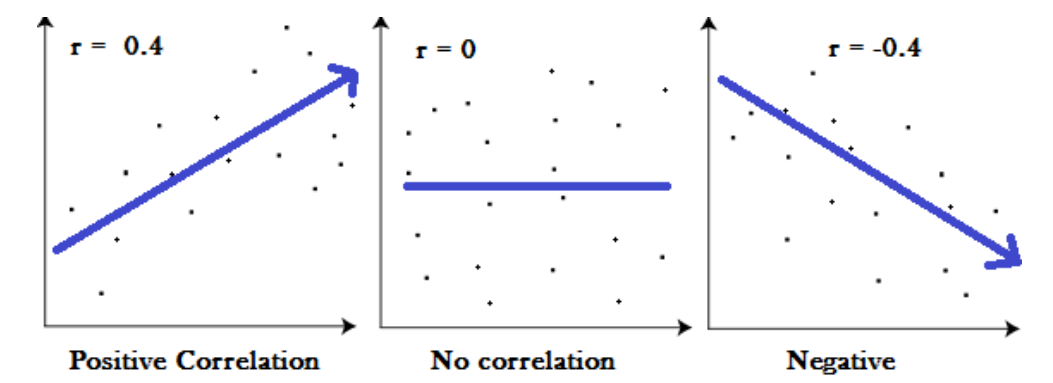
\includegraphics[width=0.5\textwidth]{Correlation Coefficient.png}
    \caption{Correlation Coefficient \protect\footnote{Source: \protect\url{https://www.statisticshowto.com/probability-and-statistics/correlation-coefficient-formula/\#Pearson}}}
    \label{fig:correlation}
\end{figure}
\end{itemize}
\subsection*{(b)} \textbf{Question:} George starts with the joint distribution (X, Y ). He finds the marginal distribution
for Y . George checks his work, and finds that the sum of the marginal distribution
probabilities is equal to 1.25. Is this correct or was an error made (is there enough
information to tell?)? If an error was made, what should be the sum of the marginal
distribution probabilities?
\begin{itemize}
    \item[] \textbf{Answer:} Yes, he made an error because the sum of the marginal distribution should be equal to 1. 
    \item[] \textbf{Explanation:} The reason for this is because if you're looking for the probability of something happening if you had a 100\% chance of something happening, that would equal 1.
    \item[] \textbf{Equation:}
    \begin{equation*}
        \begin{aligned}
        \sum_{i=1}^{n} P(Y_i) = 1
        \end{aligned}
    \end{equation*}
\end{itemize}
\newpage
\section*{Question 4}
\textbf{Question:} Random Variables:
\subsection*{(a)} \textbf{Question:} What does it mean to "define a random variable"?
\begin{itemize}
    \item[] \textbf{Answer:} To define a random variable is to assign a numerical value to each outcome of a random experiment.
    \item[] \textbf{Example:} For example, if you were to roll a die, you could define a random variable $X$ as the number that comes up when you roll the die. 
    and you can define $X$ as the set of all possible outcomes of the die roll. Such that $X = \{1, 2, 3, 4, 5, 6\}$. You could also have another die lets call that 
    $Y$ and $Y = \{1, 2, 3, 4, 5, 6\}$. You can also take those two random variables and add them together to get a new random variable $Z = X + Y$. These are all 
    examples of discrete random variables. So, if you were to roll the die and get a 1, then $X = 1$ and $Y = 1$ and $Z = 2$. The probability of getting $Z = 2$ can be expressed as $P(Z = 2)$.
    \begin{equation*}
        \begin{aligned}
        &P(Z = 2) = P(X = 1, Y = 1) \\
        &P(Z = 2) = P(X = 1) \cdot P(Y = 1) \\
        &P(Z = 2) = \frac{1}{6} \cdot \frac{1}{6} \\
        &P(Z = 2) = \frac{1}{36} \\
        \end{aligned}
    \end{equation*}
    \item[] \textbf{Conclusion:} Given our random variables $X$ and $Y$, I can define a new random variable $Z = X + Y$.
\end{itemize}
\subsection*{(b)} \textbf{Question:} Explain, in your own words, why it is important that we define a random variable
before we do any calculations. 
\begin{itemize}
    \item[] \textbf{Answer:} It is important to define a random variable before we do any calculations because it allows us to keep track of our work and simplifies expressions to make them easier to work with.
\end{itemize}
\subsection*{(c)} \textbf{Question:} When defining a random variable, we have to state the parameters. Define “parameter” using your own words.
\begin{itemize}
    \item[] \textbf{Answer:} A parameter is the logical operator that is used to define the what the random variable is including. I always think of a number line and if it is less then, equal to greater than etc.
    \item[] \textbf{Example:} Lets reuse the example with the dice, again my set is defined by $X=\{1, 2, 3, 4, 5, 6\}$ and $Y=\{1, 2, 3, 4, 5, 6\}$. If I wanted to define a new random variable $Z = X + Y$ However, I 
    wanted to only include the numbers that are less then or equal to 4 for my set of $X$ I would have to rewrite my equation for $Z$ as $Z = X + Y$ such that $X \leq 4$.
    \begin{equation*}
        \begin{aligned}
        &P(Z = 2) = P(X \leq 4, Y = 1) \\
        &P(Z = 2) = P(X \leq 4) \cdot P(Y = 1) \\
        &P(Z = 2) = \frac{2}{3} \cdot \frac{1}{6} \\
        &P(Z = 2) = \frac{1}{9} \\
        \end{aligned}
    \end{equation*}
    \item[] \textbf{Conclusion:} Parameters shape the equation and the set of possible outcomes for the random variable.
    \end{itemize}
    \newpage
\section*{Question 5} Binomial Distribution). Suppose X ~ Bin(n, p). Marcy defines a new random variable,
X/n, where n is the same constant integer as in the distribution for X.
\subsection*{(a)} \textbf{Question:} Use properties of expected value to help Marcy find E(X/n). Fully simplify your
answer (should not have an expected value in it).
\begin{itemize}
    \item[] \textbf{Answer:} 
    \begin{equation*}
        \begin{aligned}
        E(X/n) &= \frac{1}{n}E(X) \\
        &= \frac{1}{n} \cdot n \cdot p \\
        &= p
        \end{aligned}
    \end{equation*}
    \textbf{Conclusion:} The expected value of $X/n$ is $p$.
\end{itemize}
\subsection*{(b)} \textbf{Question:} Use properties of variance to help Marcy find V(X/n). Fully simplify your answer
(should not have a variance in it).
\begin{itemize}
    \item[] \textbf{Answer:} 
    \begin{equation*}
        \begin{aligned}
        V(X/n) &= \frac{1}{n^2}V(X) \\
        &= \frac{1}{n^2} \cdot n \cdot p \cdot (1 - p) \\
        &= \frac{p \cdot (1 - p)}{n}
        \end{aligned}
    \end{equation*}
    \textbf{Conclusion:} The variance of $X/n$ is $\frac{p \cdot (1 - p)}{n}$.
\end{itemize}
\newpage
\section*{Question 6} For the following problems, write down how you would code the probabilities requested into
R. You should use the specialized distribution functions mentioned in the lecture notes
from Sections 5.2–5.5. There is one problem for each distribution (Binomial, Poisson,
Geometric, and Hypergeometric). You do not need to provide the final answer. It is fine
to hand-write your code.
\subsection*{(a)} \textbf{Question:} Suppose X ~ Bin(11, 0.3). Find $P(X < 5)$
\begin{itemize}
    \item[] \textbf{Answer:} 
    \begin{figure}[h]
        \centering
        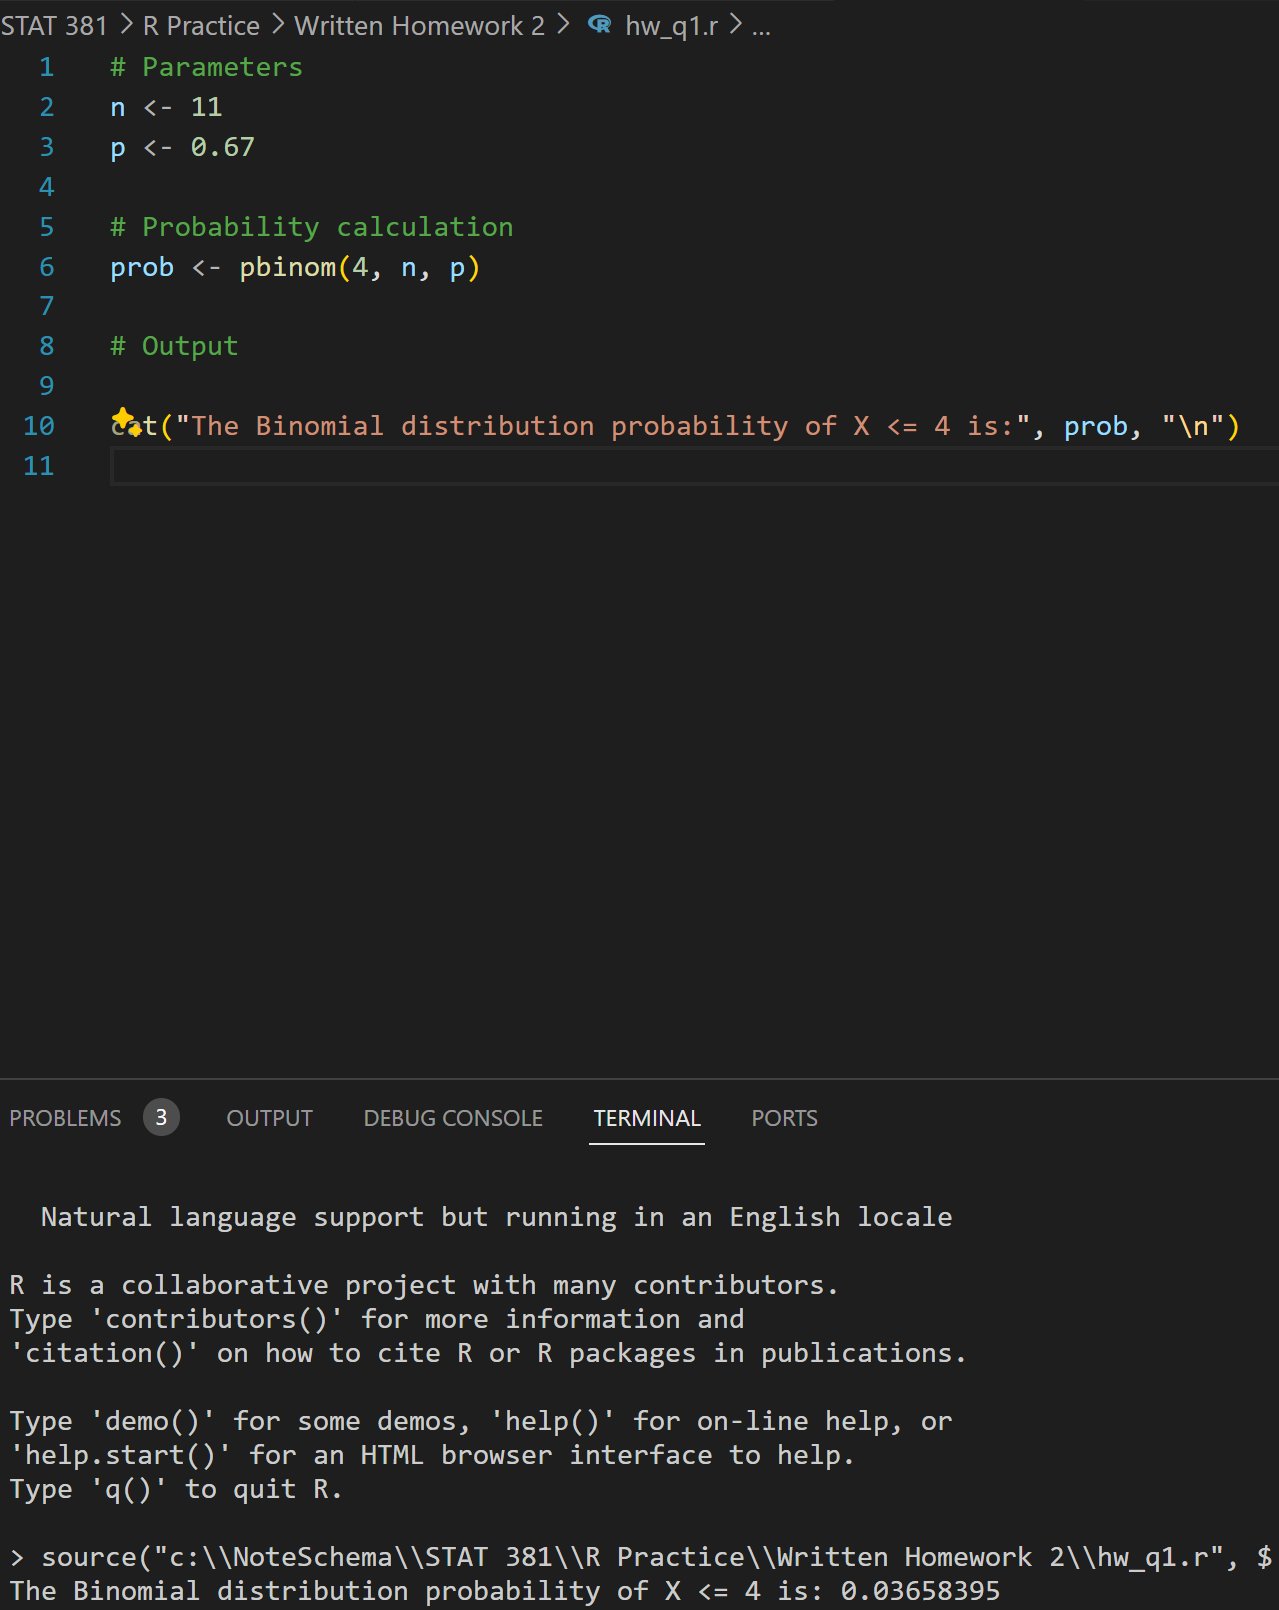
\includegraphics[width=0.5\textwidth]{RHW2.6.a.png}
        \caption{R Code for $P(X < 5)$}
        \label{fig:RHW2.6.a}
    \end{figure}
\end{itemize}
\subsection*{(b)} \textbf{Question:} Suppose a truck of books shipped to the Chicago Public Library contains 600 books.
For some reason, there are 47 books that have water damage. The librarian randomly
chooses 21 books for inspection. What is the probability that 2 or less of the inspected
books have water damage?
\begin{itemize}
    \item[] \textbf{Answer:} 
    \begin{figure}[h]
        \centering
        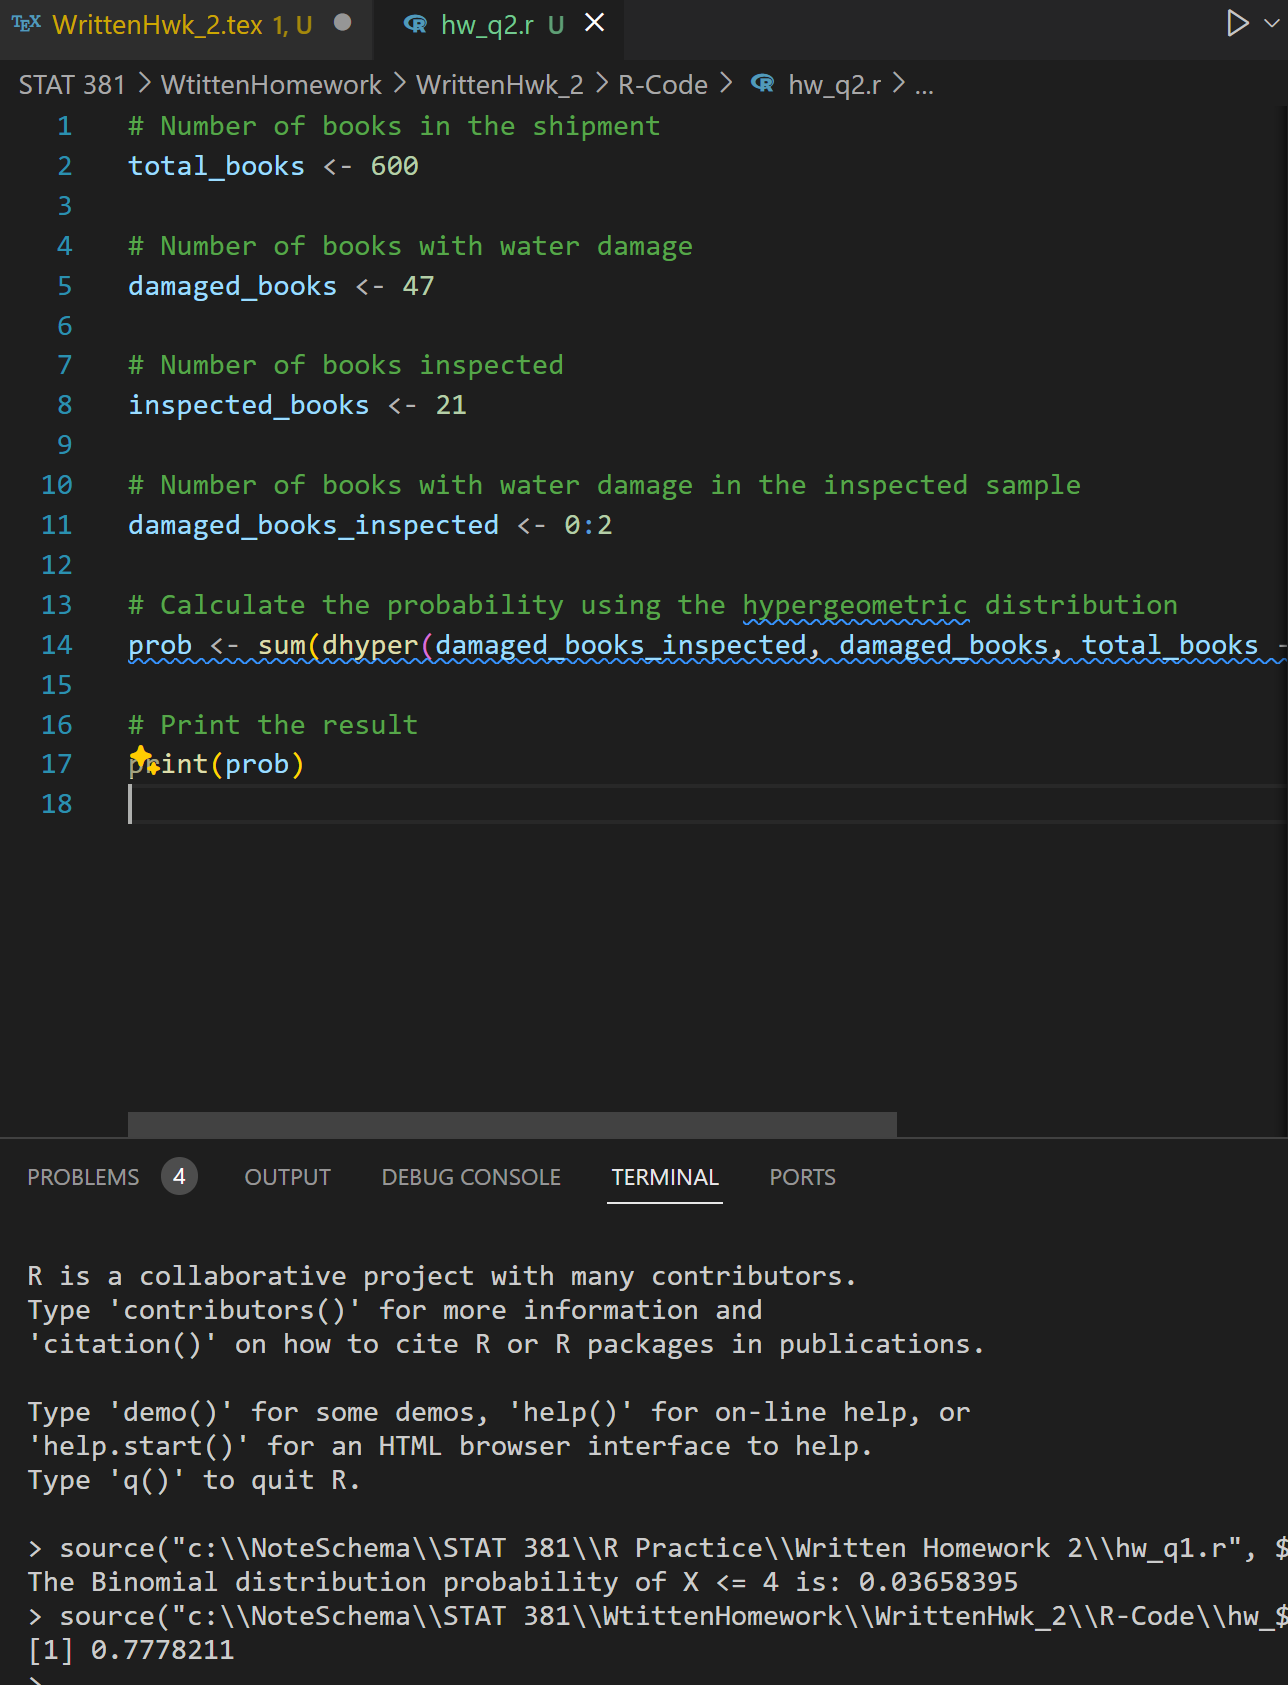
\includegraphics[width=0.5\textwidth]{RHW2.6.b.png}
        \caption{R Code for $P(X \leq 2)$}
        \label{fig:RHW2.6.b}
    \end{figure}
\end{itemize}
\newpage
\subsection*{(c)} \textbf{Question:} Suppose X ~ $Pois(\lambda t = 11)$. Find $P(X \geq 5)$ incorporating the lower tail in your calculation.
\begin{itemize}
    \item[] \textbf{Answer:} 
    \begin{figure}[h]
        \centering
        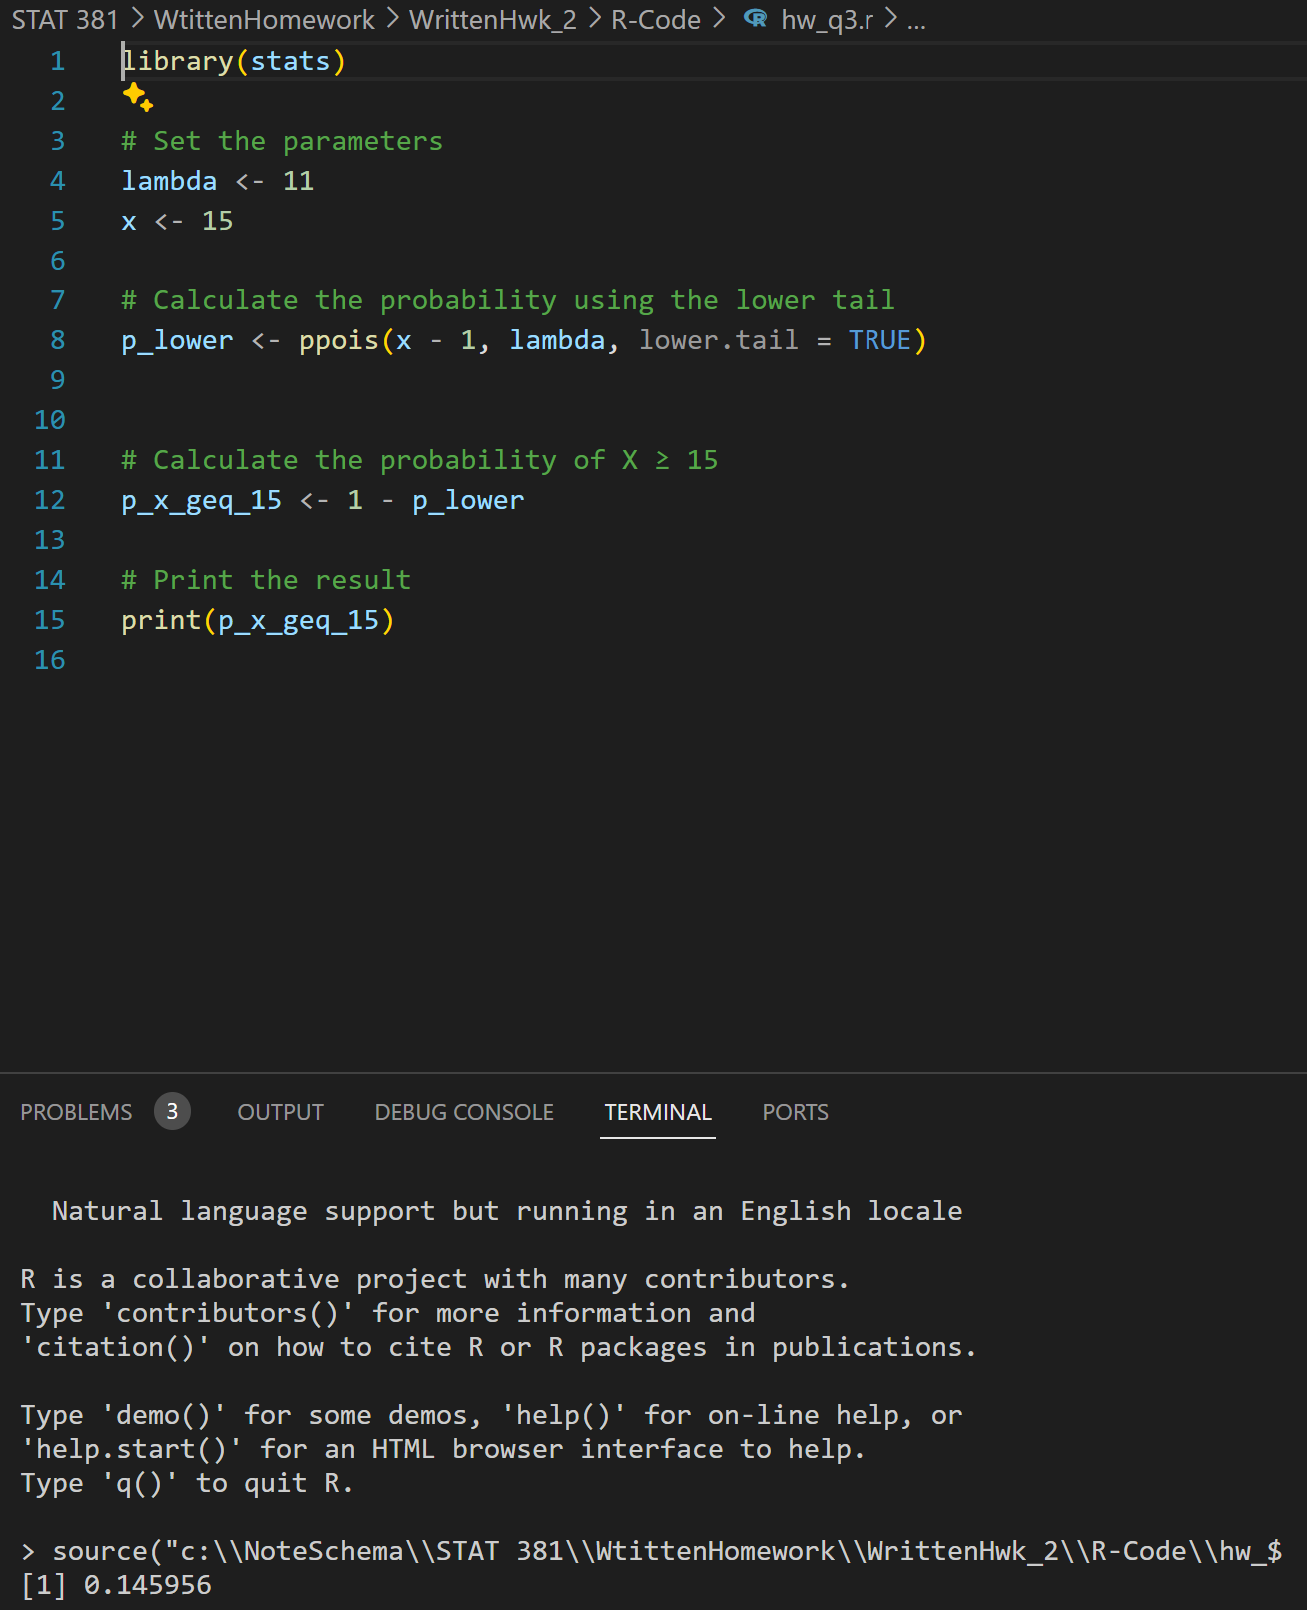
\includegraphics[width=0.5\textwidth]{RHW2.6.c.png}
        \caption{R Code for $P(X \geq 15)$}
        \label{fig:RHW2.6.c}
    \end{figure}
\end{itemize}
\newpage
\subsection*{(d)} \textbf{Question:} Suppose X ~ $Geom(p = 0.11)$. Define X to be like we did in section 5.4 class notes on page 1. We want to fin $P(X = 3)$.
\begin{itemize}
    \item[] \textbf{Answer:} 
    \begin{figure}[h]
        \centering
        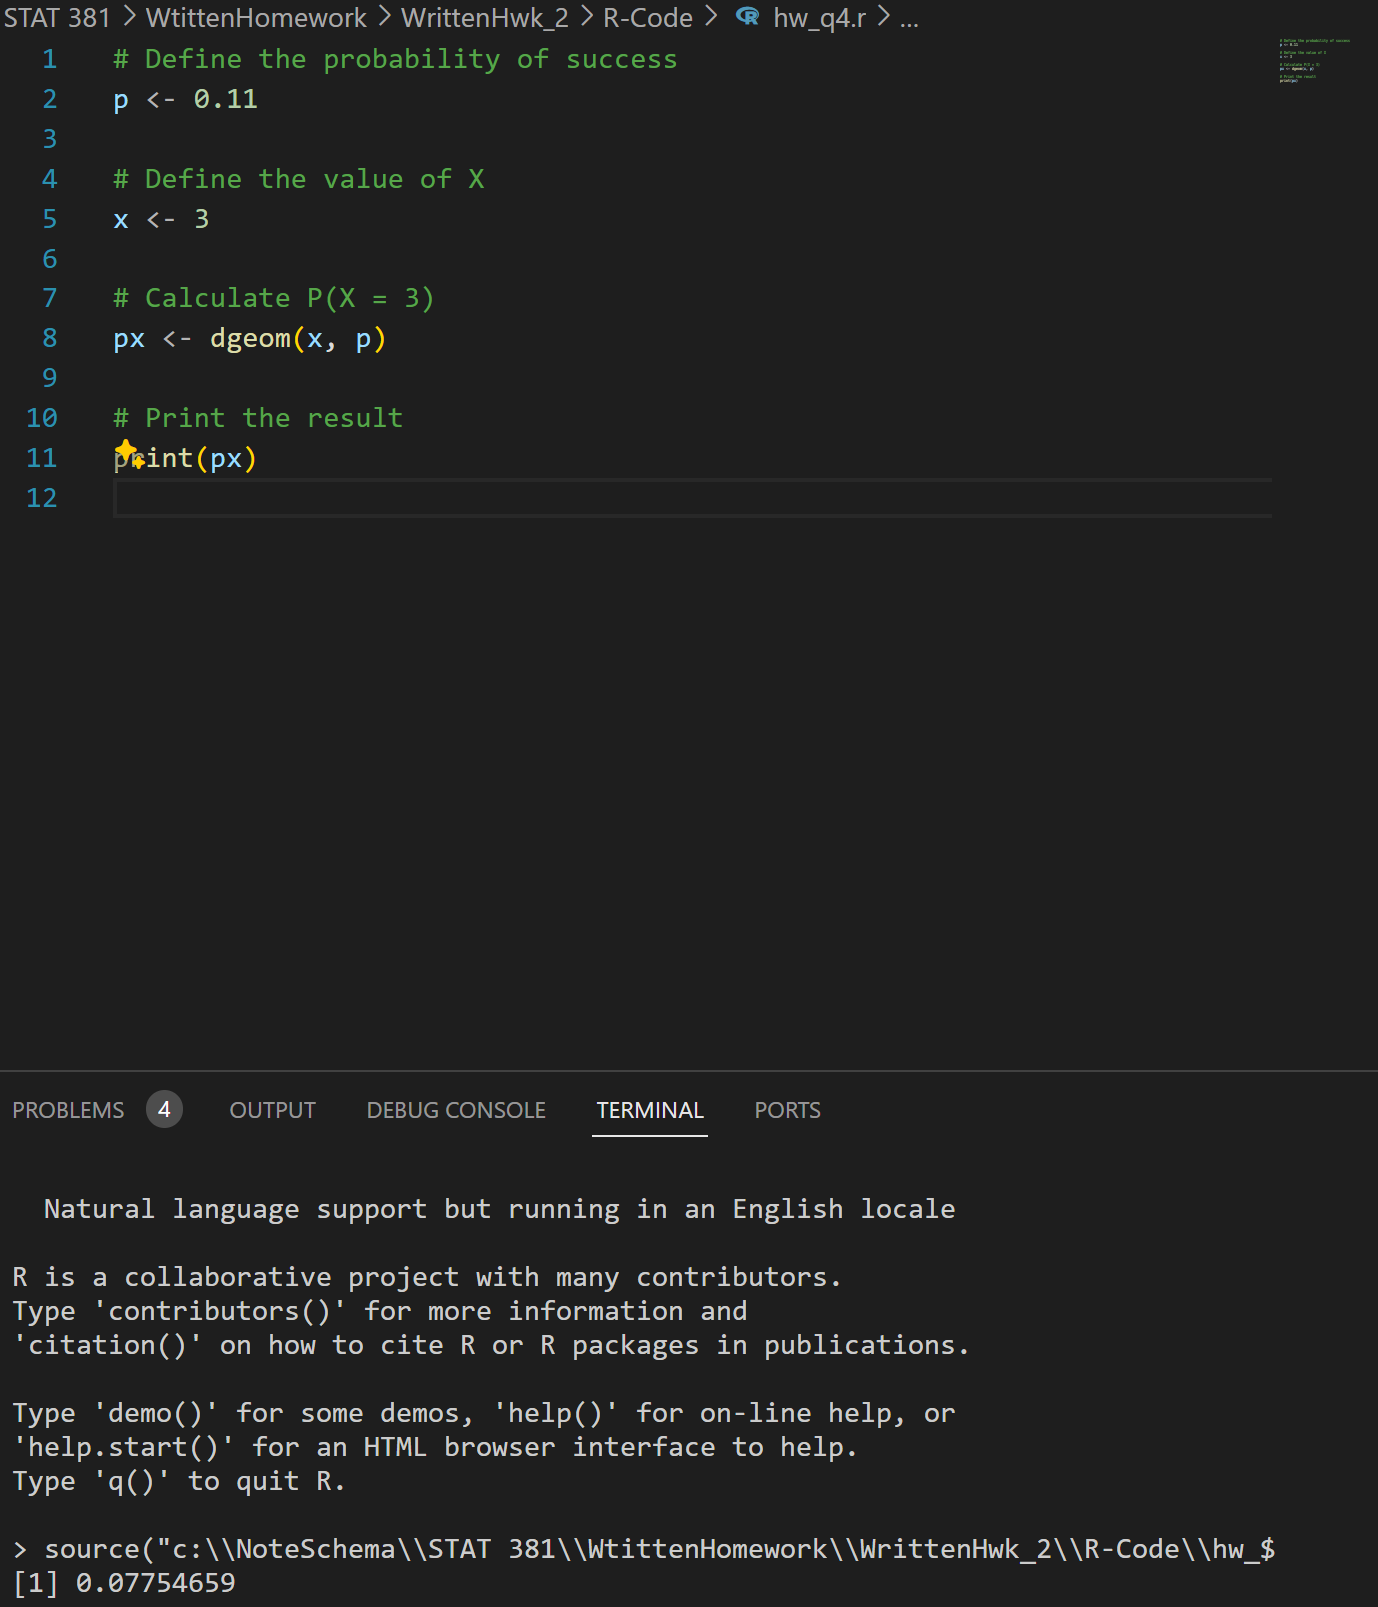
\includegraphics[width=0.5\textwidth]{RHW2.6.d.png}
        \caption{R Code for $P(X = 3)$}
        \label{fig:RHW2.6.d}
    \end{figure}
\end{itemize}
\end{document}